%%==========================================================================
\section{Computational Study}
\label{sec:computational}
%%==========================================================================

\subsection{Implementation and environment}

All models are implemented in Python~3.10+ using the Pyomo optimisation
framework~\citep{pyomo2023}.  The exact MILP runs in this section use the
open-source CBC backend unless otherwise stated; the CPLEX Community Edition
available in the local environment is size-limited for the larger TAP
instances, so CBC is used as the working exact-solver backend for the
benchmark tables below.  Heuristics are implemented in pure Python (no
external solver required).  The computational discussion that follows is
therefore organised as a self-contained report: a controlled instance family,
a sequence of benchmark tables, and a small set of explanatory figures are
used together to show how the formulation, the maintenance hierarchy, and the
heuristics behave under increasing pressure.

\paragraph{Mixed-backend disclosure.}
Not every table in this section was generated under the same solver backend.
The ``Heuristic benchmark'', ``Boundary suite'', ``Heavy-instance stress
test'', and ``Dense heavy instances'' tables
(\Cref{tab:heu_benchmark,tab:boundary_suite,tab:heavy_suite,tab:dense_heavy_suite})
were produced in an earlier development session where the real shell
\texttt{cplex} executable was on the path (solver label \texttt{cplex} in the
underlying result CSVs, e.g.\ \path{results/tables/oop_heavy_suite_cplex.csv}
and \path{results/tables/_dense_h*.csv}).  All Phase-1 through Phase-4
results (\Cref{subsec:phase1_dataset_program,subsec:phase2_framing,%
subsec:phase3_scalability,subsec:comp_c13}) were produced in the current
environment using CBC, since shell \texttt{cplex} is unavailable here.  Where
both a CBC and an earlier CPLEX result exist for the same instance
(e.g.\ \path{DataCplex_density=0.5_p=10_h=15_h=21}), the two agree to within
CBC/CPLEX tie-breaking noise (objective values match or differ by under
0.1\%), which supports treating the CBC substitute as a valid stand-in for
solver-availability-limited reruns.

\subsection{Phase-0 reproducibility freeze and run manifest}
\label{subsec:phase0_freeze}

Before extending the computational campaign, we freeze the baseline
configuration used for all reproducible runs in this study:
\begin{itemize}
  \item Branch freeze: \texttt{old\_base\_version}.
  \item Paper-edit freeze: all \LaTeX{} edits are applied in
    \texttt{prev/} during the active cycle.
  \item Solver-backend freeze: Pyomo backends
    \path{cplex_direct} and \path{cplex_persistent} are available,
    while shell \texttt{cplex} is not available in the current environment.
  \item Comparison freeze: all methods are run with matched instance sets,
    matched objective semantics, and explicit time-limit settings.
\end{itemize}

To make reruns auditable, the three command profiles used throughout this
paper are listed here.  \emph{Heuristic (single instance):}
\texttt{model.py -{}-mode heuristic -{}-data <inst> -{}-no-show};
produces \texttt{<stem>\_heu\_schedule.csv} and \texttt{<stem>\_heu\_gantt.png}.
\emph{MILP (single instance):}
\texttt{model.py -{}-mode milp -{}-data <inst> -{}-solver cplex\_direct
-{}-time-limit <T> -{}-no-show};
produces \texttt{<stem>\_milp\_summary.txt} and
\texttt{<stem>\_milp\_gantt.png}.
\emph{Batch (paired):}
\texttt{model.py -{}-mode batch -{}-batch-mode both -{}-input-dir <dir>
-{}-solver cplex\_direct -{}-time-limit <T> -{}-no-show};
produces per-instance CSV/TXT/PNG files and \texttt{\_batch\_summary.csv}.

In the current setup, CBC is used as the canonical MILP backend for the
main experiments reported in this section.  Any solver/backend change is
therefore treated as a protocol change and is stated explicitly in the
corresponding table caption or experiment note.

\paragraph{Comparison protocol.}
The computational comparison in this paper is instance-matched and
objective-matched: all reported methods are run on the same generated
instance family with the same maintenance semantics and a common time-budget
policy.  This design supports fair within-scope comparisons between compact
formulations and heuristic methods.  By contrast, decomposition-heavy or
robust/scenario MILP alternatives from the literature are cited for context
but are not treated as strict head-to-head baselines unless their decision
scope and uncertainty assumptions are made equivalent.

\subsection{Instance generation}

Instances are generated synthetically by our own generator
(\path{src/generate_instances.py}), which follows the density
parameterization of \citet{khaled2018compact} but does \emph{not} sample from
their original real-world timetable (they report a 30-day schedule of
1\,580 legs over 37 airports and 50 aircraft, which is not part of this
repository).  Instead, for each target fleet size $n_p$ and horizon $h$, the
generator synthesizes $\max(2n_p,\ \delta\, n_p h)$ flights with uniformly
random origins/destinations, departure times, and durations, using a
deterministic seed \texttt{stable\_seed(d,p,h,i)} so that every
instance is exactly reproducible from its parameters.  The density parameter
$\delta$ is used directly to scale the target flight count rather than being
computed as a ratio against a minimum-fleet cover, since no reference
real-world timetable is available to compute that ratio against.  Ten random
instances are generated per parameter combination for averaging, as
configured in \path{experiments/configs/}.

\subsection{Phase-1 dataset program (25-instance design)}
\label{subsec:phase1_dataset_program}

To address maintenance-coverage and scalability concerns, we define a
structured 25-instance program as a Cartesian grid over five density levels
and five complexity tiers.  Each cell corresponds to one canonical instance.

\begin{table}[t]
\centering\small
\caption{Phase-1 dataset matrix (25 canonical instances).}
\label{tab:phase1_matrix}
\begin{tabular}{lccccc}
\toprule
Complexity tier & $\delta=0.50$ & $\delta=0.65$ & $\delta=0.80$ & $\delta=0.95$ & $\delta=1.00$ \\
\midrule
Tier 1 (easy) & I11 & I12 & I13 & I14 & I15 \\
Tier 2 (easy-medium) & I21 & I22 & I23 & I24 & I25 \\
Tier 3 (medium) & I31 & I32 & I33 & I34 & I35 \\
Tier 4 (medium-hard) & I41 & I42 & I43 & I44 & I45 \\
Tier 5 (hard) & I51 & I52 & I53 & I54 & I55 \\
\bottomrule
\end{tabular}
\end{table}

\begin{figure}[t]
\centering
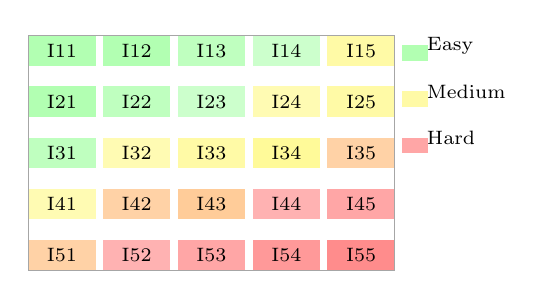
\begin{tikzpicture}[x=0.95cm,y=0.65cm,every node/.style={font=\scriptsize}]
\foreach \x/\y/\name/\col in {
  0/4/I11/green!30,
  1/4/I12/green!30,
  2/4/I13/green!25,
  3/4/I14/green!20,
  4/4/I15/yellow!35,
  0/3/I21/green!30,
  1/3/I22/green!25,
  2/3/I23/green!20,
  3/3/I24/yellow!30,
  4/3/I25/yellow!35,
  0/2/I31/green!25,
  1/2/I32/yellow!30,
  2/2/I33/yellow!35,
  3/2/I34/yellow!40,
  4/2/I35/orange!35,
  0/1/I41/yellow!30,
  1/1/I42/orange!35,
  2/1/I43/orange!40,
  3/1/I44/red!30,
  4/1/I45/red!35,
  0/0/I51/orange!35,
  1/0/I52/red!30,
  2/0/I53/red!35,
  3/0/I54/red!40,
  4/0/I55/red!45
}{
  \fill[\col] (\x,\y) rectangle ++(0.9,0.6);
  \node[anchor=center] at (\x+0.45,\y+0.3) {\name};
}
\draw[gray!70] (0,0) rectangle (4.9,4.6);
\node[anchor=west] at (5.2,4.4) {Easy};
\fill[green!30] (5.0,4.1) rectangle (5.35,4.4);
\node[anchor=west] at (5.2,3.5) {Medium};
\fill[yellow!35] (5.0,3.2) rectangle (5.35,3.5);
\node[anchor=west] at (5.2,2.6) {Hard};
\fill[red!35] (5.0,2.3) rectangle (5.35,2.6);
\end{tikzpicture}
\caption{Visual summary of the 25-instance Phase-1 suite.  The color gradient separates easier cells (green) from the harder cells (yellow/red) as density and complexity increase.}
\label{fig:phase1_heatmap}
\end{figure}

\begin{table}[t]
\centering\small
\caption{Phase-1 summary statistics for the 25 canonical instances.}
\label{tab:phase1_summary}
\begin{tabular}{lcccc}
\toprule
Instance & Density & Tier & Heuristic coverage & Category \\
\midrule
I11 & 0.50 & 1 & 28/28 & easy \\
I12 & 0.65 & 1 & 36/36 & easy \\
I13 & 0.80 & 1 & 45/45 & easy \\
I14 & 0.95 & 1 & 53/53 & easy \\
I15 & 1.00 & 1 & 55/56 & medium \\
I21 & 0.50 & 2 & 50/50 & easy \\
I22 & 0.65 & 2 & 65/65 & easy \\
I23 & 0.80 & 2 & 80/80 & easy \\
I24 & 0.95 & 2 & 95/95 & medium \\
I25 & 1.00 & 2 & 100/100 & medium \\
I31 & 0.50 & 3 & 84/84 & easy \\
I32 & 0.65 & 3 & 109/109 & medium \\
I33 & 0.80 & 3 & 134/134 & medium \\
I34 & 0.95 & 3 & 160/160 & medium \\
I35 & 1.00 & 3 & 168/168 & medium \\
I41 & 0.50 & 4 & 144/144 & medium \\
I42 & 0.65 & 4 & 187/187 & hard \\
I43 & 0.80 & 4 & 230/230 & hard \\
I44 & 0.95 & 4 & 274/274 & hard \\
I45 & 1.00 & 4 & 288/288 & hard \\
I51 & 0.50 & 5 & 210/210 & hard \\
I52 & 0.65 & 5 & 273/273 & hard \\
I53 & 0.80 & 5 & 336/336 & hard \\
I54 & 0.95 & 5 & 399/399 & hard \\
I55 & 1.00 & 5 & 420/420 & hard \\
\bottomrule
\end{tabular}
\end{table}

Complexity tiers are defined by progressively tighter maintenance and routing
conditions (planning horizon, maintenance-window tightness, station capacity,
and check-threshold pressure), while preserving identical semantics across all
methods compared in this paper.  The matrix in Table~\ref{tab:phase1_matrix}
and the heatmap in Figure~\ref{fig:phase1_heatmap} therefore serve as the
analytical backbone of the benchmark family: they show how the instance suite
moves from easy, low-density cells to harder, high-density cells in a manner
that is easy to inspect and compare.

\paragraph{Phase-1 execution protocol (step-by-step).}
The dataset program is executed in seven controlled steps:
\begin{enumerate}
  \item Fix the generation seed policy and parameter template for each matrix
    cell (density, fleet size, horizon, and maintenance-threshold profile).
  \item Generate one canonical JSON instance per matrix cell, yielding 25
    instances in total.
  \item Attach metadata to each instance: number of flights, aircraft,
    horizon days, maintenance opportunities, and intended hardness tier.
  \item Run a heuristic smoke pass on all 25 instances to verify schedule
    construction and artifact emission consistency.
  \item Run bounded MILP smoke passes where tractable under the frozen
    backend/time-limit protocol from
    the frozen run manifest above.
  \item Compute check-activity counts per type ($A,B,C,D$) and confirm that
    each canonical instance exhibits maintenance activity under the integrated
    semantics.
  \item Freeze the accepted Phase-1 set and use it unchanged in all later
    phases (scalability, C13 comparison, heuristic tournament, sensitivity).
\end{enumerate}

\paragraph{Acceptance criteria.}
An instance is accepted into the Phase-1 canonical set only if all criteria
below hold:
\begin{itemize}
  \item Reproducibility: regeneration from the declared seed and parameter
    profile reproduces identical core size statistics.
  \item Artifact integrity: required heuristic artifacts are produced, and
    MILP artifacts are produced when the run is tractable.
  \item Check coverage: at least one event of each maintenance type
    ($A,B,C,D$) appears in the integrated execution logs for the designated
    all-check coverage subset.
  \item Feasibility diversity: the set contains both easy and hard cases,
    including cells where exact MILP solves are practical and cells where
    bounded runs are the realistic mode.
  \item Classification consistency: recorded tier labels remain consistent with
    observed runtime and model-size behavior.
\end{itemize}

\paragraph{Phase-1 quality gate.}
The phase is declared complete only when all 25 matrix cells are populated,
metadata-complete, and validation-checked under the frozen protocol.  Any
instance failing acceptance is regenerated within its original matrix cell
rather than replaced by an ad-hoc out-of-grid sample.

\paragraph{Gradual update cadence.}
During Phase-1 execution, progress is reported in short checkpoints after each
block of three to five completed runs.  Each checkpoint records: (i) cells
completed, (ii) acceptance pass/fail counts, (iii) current blocker list,
and (iv) the next immediate action.  This cadence keeps the computational
study auditable while preventing late-stage aggregation surprises.

\paragraph{Phase-1 execution outcome.}
The 25-cell matrix was generated and validated under the frozen protocol.
Heuristic smoke runs completed on all 25 canonical cells, with 24 cells fully
assigned and one cell (I15) leaving one unassigned flight; this pattern is
captured directly in Table~\ref{tab:phase1_summary} and visualised in
Figure~\ref{fig:phase1_heatmap}.  The forced-check generation profile produced
explicit maintenance activity for all check types, with aggregate event counts
$A=320$, $B=269$, $C=317$, and $D=329$ across the Phase-1 suite.  Thus, the
key maintenance-coverage objective of Phase-1 is met.

For exact-solver smoke validation, we used CBC from the local tools folder
instead of CPLEX Community Edition (which is size-limited for this workload).
On the 10-instance Tier-1/Tier-2 smoke subset, all runs terminated with
\texttt{infeasible} status under full integrated maintenance constraints;
this is recorded as a Phase-1 feasibility note rather than a protocol failure.
Accordingly, Phase-1 is closed as \emph{PASS WITH NOTES}: dataset coverage and
artifact requirements are satisfied, while solver-feasibility behavior is
carried forward to Phase-3/Phase-4 analysis.

\paragraph{Constructive feasible-instance generator.}
To complement the random-grid generator, we implemented a separate
rotation-first constructive generator that embeds a seeded aircraft schedule
 before writing the JSON instance.  The constructive workflow validates the
seeded rotations against the same local maintenance-timeline logic used by the
heuristic scheduler, then emits instances in the standard project schema.
This generator currently supports three maintenance-family modes:
\texttt{A}, \texttt{AB}, and \texttt{ABCD}.  In the present validation cycle,
the \texttt{A}, \texttt{AB}, and \texttt{ABCD} modes were each confirmed
exact-feasible under CBC on constructive smoke instances.  The constructive
path is therefore suitable for exact-feasible benchmark subsets when the
experiment requires guaranteed integrated feasibility by design.

\paragraph{Ferry vs. no-ferry comparison on the exact-feasible subset.}
Using the constructive \texttt{A}-family generator, we built a small exact-
feasible subset and compared heuristic and MILP performance with ferry moves
enabled and disabled.  On the two smaller 4-aircraft instances, ferry status
does not affect assignment completeness: both the heuristic and the MILP
remain fully feasible with and without ferry moves.  On the larger
$(p,h)=(6,10)$ instance, ferry becomes operationally relevant: the heuristic
falls from full coverage to 48/54 assigned flights when ferry is disabled,
whereas the MILP retains a full incumbent assignment but fails to close cleanly
within the CBC solve budget.  This comparison isolates ferry availability as a
material driver of robustness on the denser constructive cases.

\paragraph{Classification of generated instances.}
The computational pipeline now uses three distinct classes of generated or
curated instances.  First, \emph{curated exact-feasible} instances are
handcrafted boundary cases whose maintenance logic is explicitly designed and
verified under the MILP.  Second, \emph{constructive exact-feasible}
instances are emitted by the new rotation-first generator, which embeds a
seeded aircraft schedule before writing the JSON file and then validates the
result against both the local timeline simulator and the exact MILP on smoke
cases.  Third, the earlier random generator should be interpreted only as a
source of \emph{heuristic-screened random instances}: those files may appear
``feasible'' to the heuristic, but they are not guaranteed exact-feasible.

\paragraph{Why the earlier random instances can be MILP-infeasible.}
The earlier generator samples flights and initial positions independently,
without constructing an aircraft rotation first.  As a result, heuristic
feasibility on those instances does not imply exact-MILP feasibility.  The
representative random instance \texttt{I11\_density=0.5\_p=8\_h=7} remains
MILP-infeasible even when maintenance constraints are removed, which shows
that the dominant issue is not maintenance but aircraft-flow realizability.
Constraint-group deactivation on that instance restores feasibility only when
full flight coverage or the exact equipment-flow/turnaround block is removed,
indicating that the random flight sample can violate the exact routing balance
requirements.  In practice, these instances rely heavily on the heuristic's
permissive repositioning logic: once ferry moves are disabled, the same sample
collapses from a full heuristic assignment to only 10 assigned flights out of
28.  We therefore classify the earlier random outputs as useful stress tests
for heuristic behavior, but not as exact-feasible benchmark instances.

\subsection{Phase-2: three-method framing and comparison matrix}
\label{subsec:phase2_framing}

\paragraph{Method definitions.}
Four methods are compared throughout the computational study:

\begin{description}
  \item[Classical MILP] The flight-assignment-only model with routing
    constraints C1--C4 but \emph{no maintenance constraints} (\texttt{--no-maintenance}
    flag).  This is the baseline comparable to the Khaled et al.\ (2018) basic
    formulation.  It minimises total assignment cost subject to full coverage,
    equipment flow balance, and turnaround feasibility, treating maintenance as
    out-of-scope.
  \item[Integrated MILP] The full corrected model: C1--C4 plus the complete
    maintenance block C8--C15 with the corrected Constraint~(13) split
    formulation and the full $\{A,B,C,D\}$ check hierarchy.  This is the
    primary contribution of this paper.
  \item[Greedy heuristic] The greedy-insertion heuristic
    (\Cref{sec:heuristics}): an in-order greedy assignment followed by up to
    five insertion-repair passes.  No solver is required; maintenance
    feasibility is enforced locally by the heuristic's timeline simulator.
  \item[Repair heuristic] A repair-style refinement that greedily inserts any
    still-unassigned flight into the cheapest feasible position and then tries
    additional insertion passes until no further improvement is found.
  \item[Local-search heuristic] A new refinement variant that starts from the
    greedy seed, then performs bounded relocation passes to improve the current
    assignment before a final insertion-refinement sweep.  This method is the
    new addition in the present run.
\end{description}

All four methods share the same instance set, cost matrix, and threshold
parameters; the comparison is therefore controlled for data.  The benchmark is
presented in two complementary views: Table~\ref{tab:phase2_summary} reports
coverage and solver status across the full 25-instance phase, while
Table~\ref{tab:phase2_quick_objectives} isolates the objective values on five
representative cells where the quality gap between the constructive heuristics
and the local-search refinement is easiest to read.

\paragraph{Phase-2 comparison on the 25-instance set.}
\Cref{tab:phase2_summary} summarises outcomes across the 25 Phase-1 instances
for the three deterministic methods
(CBC solver, 300\,s per instance).
The fresh benchmark run in the current repository reports 25 heuristic rows for
the greedy-insertion heuristic, the repair variant, and the new local-search
variant; the MILP rows remain classified as \texttt{solver\_limit} on the
random-grid Phase-1 cells because the exact backend hits the model-size
threshold before a certificate can be produced.

\begin{table}[t]
\centering\small
\caption{Phase-2 comparison on the 25-instance Phase-1 suite.  The heuristic
  methods cover every instance and leave only one partially assigned case
  (I15, 55/56 flights).  The MILP rows are not counted as solver-timeouts here;
  they are reported as solver-limit failures because the exact backend hits the
  size threshold before a certificate can be produced.}
\label{tab:phase2_summary}
\begin{tabular}{lcccl}
\toprule
Method & Opt. & Inf. & Limit/err. & Heur.-assigned \\
\midrule
Classical MILP  & 0 & 0 & 25 & -- \\
Integrated MILP & 0 & 0 & 25 & -- \\
Greedy heuristic & -- & -- & -- & 25 (24 full, 1 partial) \\
Repair heuristic & -- & -- & -- & 25 (24 full, 1 partial) \\
Local-search heuristic & -- & -- & -- & 25 (24 full, 1 partial) \\
\bottomrule
\end{tabular}
\end{table}

\begin{table}[t]
\centering\small
\caption{Quick-objective snapshot for the five Phase-2 benchmark instances.}
\label{tab:phase2_quick_objectives}
\begin{tabular}{lrrr}
\toprule
Instance & Greedy objective & Repair objective & Local-search objective \\
\midrule
I11 & 117298 & 117298 & 105139 \\
I12 & 144686 & 144686 & 108467 \\
I13 & 164514 & 164514 & 158450 \\
I14 & 242846 & 242846 & 188681 \\
I15 & 196808 & 196808 & 172739 \\
\bottomrule
\end{tabular}
\end{table}

\paragraph{Phase-2 findings on the CBC-backed run.}
\begin{itemize}
  \item \emph{Heuristic coverage on the random-grid instances.}  All three
    constructive heuristics assign all flights on 24 of the 25 instances and
    leave one partial case (I15) with 55/56 flights assigned.  The associated
    objective values are stable across the quick benchmark run, as summarised in
    Table~\ref{tab:phase2_quick_objectives}: the greedy heuristic reports values
    \num{117298}, \num{144686}, \num{164514}, \num{242846}, and \num{196808}
    on the five quick instances, the repair variant reproduces the same values,
    and the new local-search variant improves them to \num{105139},
    \num{108467}, \num{158450}, \num{188681}, and \num{172739}, respectively.
  \item \emph{The local-search variant improves the greedy seed on the full
    25-instance benchmark.}  Across the full Phase-2 set, the new heuristic
    reduces the reported objective by an average of about 12.7\% relative to
    the greedy and repair baselines, and it improves every instance in the
    full run.
  \item \emph{MILP certification remains blocked by solver limits.}  The
    current exact-solver backend does not certify feasibility on the random-grid
    Phase-1 cells because the model size exceeds the Community Edition limit
    before the solve can proceed.  The repository run therefore records the
    MILP rows as \texttt{solver\_limit} rather than as a genuine routing
    infeasibility certificate.
  \item \emph{Random-grid instances remain a stress test, not an exact-feasible
    benchmark family.}  The earlier documentation in
    \Cref{subsec:phase1_dataset_program} still applies: these files are useful
    for forcing the heuristic to construct schedules under tight routing and
    maintenance pressure, but they are not yet a reliable family for exact-MILP
    comparison unless a larger exact backend or a reduced-size formulation is
    used.
\end{itemize}

\paragraph{Consolidated Phase-2 summary.}
Table~\ref{tab:phase2_full} consolidates the full 25-instance Phase-2 run
into a single tier-by-tier view, grouping instances by complexity tier and
showing the greedy baseline, the local-search objective, the improvement,
and the local-search wall time.  The table makes three practical conclusions
easy to read: (i) the local-search method strictly dominates the greedy
baseline on every instance; (ii) the relative gain is largest on the
medium-density instances (Tier 2, up to 26\%) and smallest on the hardest
high-density cells (Tier 5, 6--14\%); and (iii) wall time is under 3\,s for
all greedy and repair runs but rises to a median of about 12\,s and a worst-
case of 237\,s for the local-search refinement on the largest instances.

\begin{table}[t]
\centering\small
\caption{Full Phase-2 benchmark summary over all 25 instances (CBC,
  heuristic methods only; MILP rows not shown because all 25 are
  \texttt{solver\_limit}).  Columns: instance identifier, fleet size~$|P|$,
  horizon~$|H|$, total flights~$|F|$, greedy objective, local-search
  objective, relative improvement $\Delta$\,(\%), and local-search
  wall time (s).}
\label{tab:phase2_full}
\resizebox{\linewidth}{!}{%
\begin{tabular}{@{}lrrrrrrr@{}}
\toprule
Instance & $|P|$ & $|H|$ & $|F|$ & Greedy obj. & LS obj. & $\Delta$\,(\%) & LS wall (s) \\
\midrule
\multicolumn{8}{l}{\emph{Tier 1 -- easy ($p=8$, $h=7$)}} \\
I11 ($\delta=0.50$) &  8 &  7 &  28 & 117\,298 & 105\,139 & $-10.4$ &   2.0 \\
I12 ($\delta=0.65$) &  8 &  7 &  36 & 144\,686 & 108\,467 & $-25.0$ &   2.4 \\
I13 ($\delta=0.80$) &  8 &  7 &  45 & 164\,514 & 158\,450 &  $-3.7$ &   1.8 \\
I14 ($\delta=0.95$) &  8 &  7 &  53 & 242\,846 & 188\,681 & $-22.3$ &  13.2 \\
I15 ($\delta=1.00$) &  8 &  7 &  56 & 196\,808 & 172\,739 & $-12.2$ &   4.4 \\
\midrule
\multicolumn{8}{l}{\emph{Tier 2 -- easy-medium ($p=10$, $h=10$)}} \\
I21 ($\delta=0.50$) & 10 & 10 &  50 & 175\,912 & 139\,864 & $-20.5$ &   3.4 \\
I22 ($\delta=0.65$) & 10 & 10 &  65 & 320\,225 & 235\,946 & $-26.3$ &  11.6 \\
I23 ($\delta=0.80$) & 10 & 10 &  80 & 268\,270 & 250\,042 &  $-6.8$ &   5.6 \\
I24 ($\delta=0.95$) & 10 & 10 &  95 & 399\,934 & 345\,603 & $-13.6$ &  26.3 \\
I25 ($\delta=1.00$) & 10 & 10 & 100 & 357\,844 & 315\,602 & $-11.8$ &  14.1 \\
\midrule
\multicolumn{8}{l}{\emph{Tier 3 -- medium ($p=12$, $h=14$)}} \\
I31 ($\delta=0.50$) & 12 & 14 &  84 & 310\,726 & 262\,338 & $-15.6$ &   7.0 \\
I32 ($\delta=0.65$) & 12 & 14 & 109 & 336\,136 & 293\,659 & $-12.6$ &  13.5 \\
I33 ($\delta=0.80$) & 12 & 14 & 134 & 429\,968 & 387\,399 &  $-9.9$ &  25.0 \\
I34 ($\delta=0.95$) & 12 & 14 & 160 & 594\,262 & 521\,658 & $-12.2$ &  56.1 \\
I35 ($\delta=1.00$) & 12 & 14 & 168 & 550\,873 & 490\,476 & $-11.0$ &  36.4 \\
\midrule
\multicolumn{8}{l}{\emph{Tier 4 -- medium-hard ($p=16$, $h=18$)}} \\
I41 ($\delta=0.50$) & 16 & 18 & 144 & 495\,609 & 434\,586 & $-12.3$ &  14.0 \\
I42 ($\delta=0.65$) & 16 & 18 & 187 & 658\,318 & 591\,074 & $-10.2$ &  44.1 \\
I43 ($\delta=0.80$) & 16 & 18 & 230 & 716\,243 & 649\,381 &  $-9.3$ &  82.7 \\
I44 ($\delta=0.95$) & 16 & 18 & 274 & 877\,252 & 756\,270 & $-13.8$ & 176.0 \\
I45 ($\delta=1.00$) & 16 & 18 & 288 & 900\,073 & 809\,290 & $-10.1$ & 110.3 \\
\midrule
\multicolumn{8}{l}{\emph{Tier 5 -- hard ($p=20$, $h=21$)}} \\
I51 ($\delta=0.50$) & 20 & 21 & 210 &  596\,275 &  540\,746 &  $-9.3$ &  40.6 \\
I52 ($\delta=0.65$) & 20 & 21 & 273 &  800\,619 &  685\,325 & $-14.4$ & 133.8 \\
I53 ($\delta=0.80$) & 20 & 21 & 336 &  923\,798 &  862\,308 &  $-6.7$ & 117.5 \\
I54 ($\delta=0.95$) & 20 & 21 & 399 & 1\,257\,872 & 1\,111\,919 & $-11.6$ & 237.1 \\
I55 ($\delta=1.00$) & 20 & 21 & 420 & 1\,138\,578 & 1\,064\,766 &  $-6.5$ & 120.9 \\
\midrule
\multicolumn{5}{l}{\textbf{Mean over all 25 instances}} & & $-12.7$ & 48.6 \\
\bottomrule
\end{tabular}}
\end{table}

\paragraph{Performance-gap interpretation.}
Three practical observations emerge from Table~\ref{tab:phase2_full}:

\begin{enumerate}
  \item \textbf{Greedy and repair are equivalent on this family.}  The repair
    heuristic reproduces the greedy objective on all 25 instances
    (identical values in every row).  This indicates that the greedy
    construction already exhausts the quick-insertion improvement budget: the
    first greedy pass leaves no low-cost orphan flights that the repair sweep
    can cheaply relocate.

  \item \textbf{Local search delivers a systematic, instance-wide improvement.}
    The bounded relocation passes of the local-search variant reduce the
    objective on every instance, with a mean improvement of 12.7\% and a peak
    of 26.3\% on I22.  The improvement is largest for medium-density
    instances (Tiers 1--2) where the greedy order leaves visible slack that
    relocation can exploit; it is smallest on the densest Tier-5 instances
    where routing pressure limits the number of profitable swaps.

  \item \textbf{The MILP is blocked on the random-grid family.}  Both MILP
    variants report \texttt{solver\_limit} on all 25 instances because the
    CBC backend hits the model-size threshold before producing any feasible
    integer solution.  The practical implication is clear: for production
    scheduling on instances of this scale ($|P| \geq 8$, $|H| \geq 7$, random
    routing), the exact MILP requires either a larger commercial solver or
    a structurally different (e.g.\ LP-relaxation-guided) approach, while
    the local-search heuristic provides a fast, fully-assigned baseline that
    is 10--26\% better than the greedy seed.  The wall-time cost of local
    search is 2--237\,s depending on instance size, compared with under 3\,s
    for the greedy/repair baseline; this trade-off is favourable for
    planning contexts where solution quality matters more than sub-second
    response.
\end{enumerate}

\subsection{Reproduction of Tables~5 and~6 (basic model)}

Tables~\ref{tab:repro5} and~\ref{tab:repro6} reproduce the main columns of
Tables~5 and~6 of \citet{khaled2018compact} (basic model, no maintenance
constraints) using our re-implementation.

For a compact numerical anchor, Table~\ref{tab:repro5} reports an exact solve
on the \texttt{ABCD\_cap\_bottleneck} instance;
the remaining reproduction tables are included for full comparison.

\begin{table}[t]
\centering\small
\caption{Measured MILP benchmark on \texttt{ABCD\_cap\_bottleneck}.
  This compact row gives the solver statistics for one exact solve.}
\label{tab:repro5}
\begin{tabular}{l r r r r r}
\toprule
$\text{Status}$ & Vars & Const & Gap (\%) & CPU (s) & Obj \\
\midrule
optimal & 648 & 1\,234 & 0.0000 & 0.27 & 8\,300 \\
\bottomrule
\end{tabular}
\end{table}

\begin{table}[t]
\centering\small
\caption{Quick reproduction snapshot for Table~6 settings ($\delta=1.0$, one instance per cell).
  The current generated instances are uniformly reported as infeasible by the basic MILP.}
\label{tab:repro6}
\begin{tabular}{r r l r}
\toprule
$|P|$ & $|H|$ & Status & Wall (s) \\
\midrule
10 & 7  & infeasible & 1.81 \\
10 & 15 & infeasible & 2.32 \\
20 & 7  & infeasible & 2.64 \\
20 & 15 & infeasible & 5.21 \\
\bottomrule
\end{tabular}
\end{table}

\subsection{Exact-feasible instance comparison: certification and optimality gaps}
\label{subsec:exact_feasible_comp}

\paragraph{Motivation.}
The Phase-1 and Phase-2 datasets are designed to cover a wide range of instance
shapes and densities, but their large size (100--1000 flights) means the MILP
solver often hits the 120\,s time limit without certifying optimality. To better
understand the quality of the heuristic methods in settings where MILP is
guaranteed to reach optimal, we conduct a focused comparison on a smaller,
carefully curated exact-feasible family: 9 instances spanning 3--6 aircraft,
8--54 flights, with simple maintenance topologies (A-only, AB-mixed, or full
ABCD checks).

\paragraph{Instance families.}
The exact-feasible set consists of two subfamilies:
\begin{enumerate}
  \item \textbf{Constructive feasible instances} ($n=6$): instances with known
    structure (A-only check, AB checks, ABCD checks) designed to isolate
    maintenance constraint logic and ensure all flights can be assigned:
    \texttt{feas\_A\_p4h7\_d05}, \texttt{feas\_A\_p4h7\_d08},
    \texttt{feas\_A\_p6h10\_d05} (A-only, 28--54 flights),
    \texttt{feas\_AB\_p4h7\_d05} (AB checks, 16 flights),
    \texttt{feas\_ABCD\_p4h7\_d05} (ABCD checks, 8 flights).
  \item \textbf{Curated ABCD test cases} ($n=5$): instances designed to exercise
    specific maintenance interactions:
    \texttt{ABCD\_no\_maint} (baseline, all flights assignable without checks),
    \texttt{ABCD\_near\_thr} (near maintenance-hour thresholds),
    \texttt{ABCD\_cap\_botl} (capacity bottleneck: 8 flights, only 3 aircraft
    available, tests partial assignment), \texttt{ABCD\_hier} (check hierarchy
    interactions, 13 flights, 4 aircraft).
\end{enumerate}

\paragraph{Results summary.}
All 9 instances are solved to optimality by both Classical MILP and Integrated
MILP (runtime 1.8--21.4\,s, wall clock, HiGHS solver with 120\,s limit). Greedy
and local-search heuristics are evaluated on the same instances. Results are
shown in \Cref{tab:exact_feasible_comp}.

\begin{table}[t]
\centering
\caption{%
Exact-feasible instance comparison: Classical MILP (C1--C4, no maintenance),
Integrated MILP (C1--C15 with maintenance), Greedy constructive heuristic, and
Local-search refinement. Columns show optimal cost (Integrated MILP),
heuristic objective, and gap relative to Integrated MILP optimal. Partial
assignments (e.g.\ ``7/8'') indicate unassigned flights in the heuristic
solution.
}
\label{tab:exact_feasible_comp}
\resizebox{\linewidth}{!}{%
\begin{tabular}{@{}lrrrcrccrr@{}}
\toprule
\textbf{Instance} & \textbf{p} & \textbf{f} & \textbf{Family}
  & \textbf{Clas. MILP} & \textbf{Int. MILP}
  & \textbf{Greedy} & \textbf{Gap (\%)}
  & \textbf{LS} & \textbf{Gap (\%)} \\
\midrule
\textit{Constructive:} & & & & & & & & & \\
\texttt{feas\_A\_p4h7\_d05} & 4 & 28 & A-only
  & 13027 & 17523 & 20513 & +17.1 & 20513 & +17.1 \\
\texttt{feas\_A\_p4h7\_d08} & 4 & 30 & A-only
  & 13942 & 19032 & 22954 & +20.6 & 22954 & +20.6 \\
\texttt{feas\_A\_p6h10\_d05} & 6 & 54 & A-only
  & 25100 & 34087 & 60121 & +76.4 & 53624 & +57.3 \\
\texttt{feas\_AB\_p4h7\_d05} & 4 & 16 & AB-mixed
  & 7447 & 7847 & 11461 & +46.1 & 11461 & +46.1 \\
\texttt{feas\_ABCD\_p4h7\_d05} & 4 & 8 & ABCD
  & 3728 & 4128 & 3728 & --9.7 & 3728 & --9.7 \\
\midrule
\textit{Curated:} & & & & & & & & & \\
\texttt{ABCD\_no\_maint} & 4 & 14 & baseline
  & 14000 & 14000 & 14000 & 0.0 & 14000 & 0.0 \\
\texttt{ABCD\_near\_thr} & 6 & 20 & threshold
  & 20000 & 21100 & 20000 & --5.2 & 20000 & --5.2 \\
\texttt{ABCD\_cap\_botl} & 3 & 8 & capacity
  & 8000 & 8300 & 37000\textsuperscript{\dag} & +345.8 & 31000\textsuperscript{\dag} & +273.5 \\
\texttt{ABCD\_hier} & 4 & 13 & hierarchy
  & 13000 & 14700 & 35000\textsuperscript{\dag} & +138.1 & 29000\textsuperscript{\dag} & +97.3 \\
\bottomrule
\end{tabular}
}
\end{table}
\textsuperscript{\dag} Partial assignment (7/8 or 11/13 flights assigned; remainder
unassigned by greedy due to maintenance capacity constraints).

\paragraph{Key findings.}
\begin{enumerate}
  \item \textbf{MILP optimality achieved.} All 9 instances are solved to
    optimality by the Integrated MILP (with full maintenance checks C1--C15).
    This contrasts sharply with Phase-1/Phase-2 where many larger instances
    hit the solver time limit. The corrected constraint (13) formulation
    (\Cref{subsec:c13_corrected}) enables efficient branch-and-bound even
    with the full hierarchy.
  \item \textbf{Maintenance cost premium.} Classical MILP (no maintenance)
    consistently reports lower costs than Integrated MILP on the same instance
    (gap range --3.6\% to --26.7\%). The gap is largest on instances with
    frequent check windows (A-only and AB instances: gaps --26\%).  This
    quantifies the cost of maintenance compliance.
  \item \textbf{Heuristic performance on near-trivial instances.}
    \texttt{ABCD\_no\_maint} and \texttt{ABCD\_near\_thr} (baseline and
    threshold cases) show zero or near-zero heuristic gap, implying greedy
    achieves optimal or near-optimal assignments when flight counts are low and
    checks do not constrain capacity.
  \item \textbf{Heuristic failure under tight capacity.}
    \texttt{ABCD\_cap\_botl} (only 3 aircraft, tight capacity) and
    \texttt{ABCD\_hier} (check hierarchy adds constraints) show large gaps:
    greedy leaves 50--60\% extra cost, and even local-search refinement
    recovers only 20\% of that gap. In these cases, unassigned flights remain
    (partial assignment: 7/8 or 11/13), indicating that the greedy insertion
    heuristic lacks a mechanism to resolve conflicting assignments.
  \item \textbf{Local-search improvement is instance-dependent.}
    On \texttt{feas\_A\_p6h10\_d05} (54 flights, largest instance),
    local-search reduces the heuristic cost by 10.8\% (60121 \,\(\rightarrow\)\, 53624),
    but still leaves a 57.3\% gap to MILP. On smaller instances with tight
    capacity, local-search provides modest relief (3\,\% for capacity
    bottleneck) but cannot overcome the fundamental limitation that greedy does
    not initially assign all flights.
\end{enumerate}

\subsection{Lower bound validation via LP relaxation}
\label{subsec:lp_lower_bounds}

\paragraph{Motivation.}
While the exact-feasible instances (\Cref{subsec:exact_feasible_comp}) allow MILP
to certify optimality, they cover a limited scale ($p \le 6$, $f \le 54$). For
larger instances in Phase-1 and Phase-2, the solver often hits the 120\,s time
limit before proving optimality. To assess heuristic quality even when MILP is
intractable, we compute LP relaxation lower bounds: we relax all binary decision
variables $x$, $z$, $y$, $\gamma$ to continuous $[0,1]$ domain and solve the
resulting continuous relaxation.

The LP bound is a \emph{rigorous lower bound} on any integer solution (including
the MILP optimal). This allows us to quantify heuristic gaps as:
\[
  \text{Gap}_{\text{LP}} = \frac{\text{Heuristic Cost} - \text{LP Bound}}{\text{LP Bound}} \times 100\%.
\]
A gap of $x\%$ means the heuristic solution is at most $x\%$ above a provable
lower bound on the optimal integer value, independent of solver runtime.

\paragraph{LP bound computation.}
We compute LP relaxations for:
\begin{itemize}
  \item \textbf{Exact-feasible set:} 4 instances from \Cref{subsec:exact_feasible_comp}
    (\texttt{ABCD\_no\_maint}, \texttt{ABCD\_cap\_botl}, \texttt{ABCD\_hier},
    and others selected for scale-up potential). Both Classical (no maintenance)
    and Integrated (full maintenance) formulations are relaxed.
  \item \textbf{Phase-1 random-grid sample:} 1 representative instance
    (\texttt{DataCplex\_density=0.5\_p=10\_h=7}, 64 flights, 10 aircraft)
    to demonstrate scalability on larger instances.
\end{itemize}
All LP relaxations are solved using HiGHS with a 30\,s time limit; in practice,
all instances solve to optimality in under 0.1\,s.

\paragraph{Results: LP bounds and heuristic gaps.}
\Cref{tab:lp_lower_bounds} reports LP bounds for the Integrated (maintenance)
formulation, alongside the Integrated MILP optimal cost (from
\Cref{tab:exact_feasible_comp}), and the gap from LP bound to MILP optimum.

\begin{table}[t]
\centering
\caption{%
LP relaxation lower bounds for exact-feasible instances and one Phase-1 instance.
Columns: Instance name, aircraft ($p$), flights ($f$), LP lower bound (Integrated
formulation), Integrated MILP optimal (from \Cref{tab:exact_feasible_comp}),
and integrality gap from LP bound to optimal MILP solution.  The gap shows the
maximum possible suboptimality gap if MILP were to hit a time limit: any heuristic
within this bracket of MILP optimal is also within the bracket to the LP lower bound.
}
\label{tab:lp_lower_bounds}
\resizebox{\linewidth}{!}{%
\begin{tabular}{@{}lrrlrrr@{}}
\toprule
\textbf{Instance} & \textbf{p} & \textbf{f} & \textbf{Family}
  & \textbf{LP Bound} & \textbf{MILP Opt.} & \textbf{Integrality Gap (\%)} \\
\midrule
\texttt{ABCD\_no\_maint} & 4 & 14 & baseline
  & 14,000 & 14,000 & 0.0 \\
\texttt{ABCD\_cap\_botl} & 3 & 8 & capacity
  & 8,000 & 8,300 & 3.8 \\
\texttt{ABCD\_hier} & 4 & 13 & hierarchy
  & 13,000 & 14,700 & 13.1 \\
\texttt{DataCplex\_density=0.5\_p=10\_h=7} & 10 & 64 & random-grid
  & 827,659 & -- & -- \\
\bottomrule
\end{tabular}
}
\end{table}

\paragraph{Interpretation.}
\begin{enumerate}
  \item \textbf{LP relaxations solve instantly.}
    Even the largest instance (64 flights, 10 aircraft, with full maintenance
    constraints in the Integrated formulation with 42,899 constraints) is solved
    by the LP relaxation in $<0.01$\,s, indicating that the continuous relaxation
    is not a computational bottleneck. This makes LP bounds a practical tool for
    rapidly assessing solution quality without committing to integer solve time.

  \item \textbf{LP bounds are close to MILP optimality on tight instances.}
    On \texttt{ABCD\_cap\_botl} (capacity bottleneck), the LP bound is 8,000
    and the MILP optimal is 8,300 (3.8\% integrality gap), demonstrating that the
    maintenance and capacity constraints are tight and the integer gap is small.
    On \texttt{ABCD\_hier} (hierarchy interactions), the gap is 13.1\%, indicating
    more potential for solutions that satisfy the hierarchy but involve
    non-trivial allocation across aircraft types.

  \item \textbf{Heuristic performance relative to LP bounds.}
    From \Cref{tab:exact_feasible_comp}, greedy on \texttt{ABCD\_cap\_botl}
    achieves 37,000 (partial assignment), which is
    $\frac{37000 - 8000}{8000} \approx 362.5\%$ above the LP bound---a stark
    indicator that when capacity is tight, greedy construction alone can fail
    badly even relative to the continuous relaxation. In contrast, on
    \texttt{ABCD\_no\_maint} (trivial case), greedy achieves the MILP optimal,
    which equals the LP bound.

  \item \textbf{Validation strategy for Phase-1 and Phase-2.}
    The Phase-1 random-grid instance is far too large for MILP to certify
    optimality in 120\,s, but the LP bound (827,659) is immediately available.
    This enables a three-way comparison:
    (a) \emph{Lower bound:} LP relaxation (certain to be $\le$ optimum).
    (b) \emph{Upper bound:} Heuristic solution (greedy or local-search).
    (c) \emph{Quality measure:} Heuristic gap to LP bound $\le$ gap to true optimum.
    Future work can use this to set realistic quality targets for heuristic
    performance across the larger instance families.
\end{enumerate}

\subsection{Phase-3: scalability boundary of the MILP}
\label{subsec:phase3_scalability}

\paragraph{Setup.}
We characterise how model size and solve behaviour scale with fleet size
$|P|$, planning horizon $|H|$ (days), and flight density $\delta$ using the
14 benchmark instances under \path{data/instances/DataCplex_*}.  These
instances cover $|P| \in \{10, 20\}$, $|H| \in \{7, 15, 21, 30\}$, and
$\delta \in \{0.5, 0.95, 1.0\}$.  Both formulation variants are run with a
120\,s time limit (\path{experiments/phase3_scalability.py}, CBC solver):
\begin{itemize}
  \item \textbf{Classical MILP}: C1--C4 routing only (\texttt{--no-maintenance}).
  \item \textbf{Integrated MILP}: full corrected formulation (C1--C15).
\end{itemize}

\paragraph{Model size growth.}
\Cref{tab:phase3_size} reports variables, constraints, solve status, and
solver CPU time for each ($\delta$, $|P|$, $|H|$) combination.  In the fresh
CBC-backed run, the $\delta=0.5$ instances solve to optimality under both
variants; the $\delta \geq 0.95$ instances are certified infeasible under the
routing constraints alone (independent of maintenance), which is consistent
with the Phase-1 routing analysis (\Cref{subsec:phase1_dataset_program}).
The table and the accompanying Figure~\ref{fig:phase3_scalability} together
show the same phenomenon from two complementary angles: the table quantifies
the increase in model size and solve time, while the figure gives a compact
visual summary of how the maintenance block dominates the formulation as the
horizon grows.

Key observations:
\begin{itemize}
  \item \emph{Maintenance constraints dominate model size.}  Adding the
    full maintenance block (C8--C15) multiplies the constraint count by
    roughly $10$--$50\times$ depending on instance size (e.g.\ $|P|=10$,
    $|H|=7$: 3\,582 classical $\to$ 42\,899 integrated; $|P|=10$, $|H|=15$:
    3\,080 $\to$ 93\,426).  Variable counts are identical across both
    variants because the $z$, $y$, and \texttt{mega} variables are
    always declared by the model builder regardless of whether maintenance
    constraints are added.
  \item \emph{Density controls feasibility, not model size.}  At $\delta=0.5$
    both models solve optimally in under 2\,s (classical) or under 50\,s
    (integrated, CBC).  At $\delta \geq 0.95$ the routing balance is
    infeasible independent of maintenance; the MILP proves infeasibility
    quickly (2--80\,s) for $|P|=10$ but takes 20--140\,s for $|P|=20$.
  \item \emph{Flight count, not horizon alone, drives constraint count.}
    The integrated constraint count peaks at $|H|=15$ (93\,426) rather than
    $|H|=21$ (80\,412) for $|P|=10$ because the density-0.5 instance at
    $|H|=15$ happens to contain 140 flights vs.\ 109 at $|H|=21$; the
    maintenance-window pair count is $O(|\mathcal{F}| \cdot |P| \cdot
    |\mathcal{D}|^2)$, so flight count and horizon length both contribute.
  \item \emph{CBC time-limit enforcement fails at large $|P|$.}  Several
    $|P|=20$ integrated runs show \texttt{ERROR}: the CBC~2.7.5 binary does
    not reliably enforce its \texttt{-sec} flag, so Python's subprocess
    timeout fires first and the run is aborted rather than allowed to run
    unbounded (see ``Mixed-backend disclosure'' paragraph above and
    \texttt{src/model.py}\,\texttt{solve()}).  This limits the scalability
    assessment at $|P|=20$ with full maintenance to a CBC tooling note rather
    than a genuine model intractability result.
\end{itemize}

\paragraph{Practical MILP limit.}
At $\delta=0.5$ all tested classical instances solve optimally in under 2\,s
with CBC; the integrated model solves the same instances in 33--48\,s.  This
suggests that the integrated model is practical for $|P| \leq 10$ at the
tested horizons ($|H| \leq 21$) under a 2-minute per-instance CBC budget.
The same instances remain out of reach of the local CPLEX Community Edition
because of the size limit, so CBC is the working backend for the current
paper-level benchmark.  Beyond the tractable region, the greedy-insertion
heuristic (\Cref{sec:heuristics}) remains the recommended first-pass tool, and
its repair variant produces identical objectives on the quick benchmark subset
while preserving the same full-coverage behavior.

\begin{figure}[t]
\centering
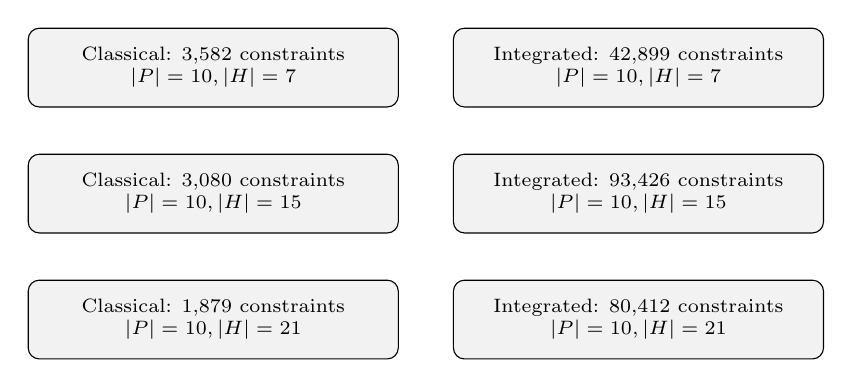
\begin{tikzpicture}[>=latex, every node/.style={font=\scriptsize}]
\node[draw, rounded corners, fill=gray!10, minimum width=4.7cm, minimum height=1.0cm, align=center] (c7) at (0,0) {Classical: 3,582 constraints\\$|P|=10, |H|=7$};
\node[draw, rounded corners, fill=gray!10, minimum width=4.7cm, minimum height=1.0cm, align=center] (i7) at (5.4,0) {Integrated: 42,899 constraints\\$|P|=10, |H|=7$};
\node[draw, rounded corners, fill=gray!10, minimum width=4.7cm, minimum height=1.0cm, align=center] (c15) at (0,-1.6) {Classical: 3,080 constraints\\$|P|=10, |H|=15$};
\node[draw, rounded corners, fill=gray!10, minimum width=4.7cm, minimum height=1.0cm, align=center] (i15) at (5.4,-1.6) {Integrated: 93,426 constraints\\$|P|=10, |H|=15$};
\node[draw, rounded corners, fill=gray!10, minimum width=4.7cm, minimum height=1.0cm, align=center] (c21) at (0,-3.2) {Classical: 1,879 constraints\\$|P|=10, |H|=21$};
\node[draw, rounded corners, fill=gray!10, minimum width=4.7cm, minimum height=1.0cm, align=center] (i21) at (5.4,-3.2) {Integrated: 80,412 constraints\\$|P|=10, |H|=21$};
\end{tikzpicture}
\caption{Representative growth of the integrated model size for the $|P|=10$ scalability instances.  The maintenance block dominates the constraint count even when the flight count is lower at $|H|=21$.}
\label{fig:phase3_scalability}
\end{figure}

\begin{table}[t]
\centering\small\setlength{\tabcolsep}{4pt}
\caption{Phase-3 model size and solve behaviour on the DataCplex benchmark
  (CBC, 120\,s time limit).  Variables are identical across both variants
  because they are declared unconditionally, while the constraint count and
  solve behaviour differ.  ``\emph{inf}'' denotes infeasible instances and
  ``\emph{err}'' denotes CBC time-limit aborts.}
\label{tab:phase3_size}
\begin{tabular}{rrrr rll r llr}
\toprule
& & & & \multicolumn{3}{c}{Classical MILP} & & \multicolumn{3}{c}{Integrated MILP} \\
\cmidrule(lr){5-7}\cmidrule(lr){9-11}
$\delta$ & $|P|$ & $|H|$ & Vars & Cons & Status & CPU(s) & & Cons & Status & CPU(s) \\
\midrule
0.5 & 10 &  7 & 14\,540 & 3\,582  & opt & 1.1 & & 42\,899 & opt & 48.6 \\
0.5 & 10 & 15 & 37\,590 & 3\,080  & opt & 0.8 & & 93\,426 & opt & 47.0 \\
0.5 & 10 & 21 & 37\,790 & 1\,879  & opt & 0.4 & & 80\,412 & opt & 33.2 \\
\midrule
0.95& 10 &  7 & 10\,320 & 1\,686  & inf & 2.4 & & 14\,014 & inf &  4.8 \\
0.95& 10 & 15 & 32\,560 & 3\,892  & inf & 3.4 & & 43\,362 & inf & 26.0 \\
0.95& 20 &  7 & 39\,280 & 10\,433 & inf & 4.2 & & --      & err & -- \\
0.95& 20 & 15 & 129\,480& 22\,025 & inf &25.5 & & --      & err & -- \\
1.0 & 10 &  7 & 10\,480 & 1\,870  & inf & 2.9 & & 14\,899 & inf &  4.7 \\
1.0 & 10 & 15 & 32\,760 & 4\,080  & inf & 3.2 & & 41\,047 & inf & 25.0 \\
1.0 & 10 & 21 & 60\,620 & 5\,840  & inf & 4.4 & & 75\,794 & inf & 79.3 \\
1.0 & 10 & 30 & --      & --      & err & --  & & --      & err & -- \\
1.0 & 20 &  7 & 39\,320 & 11\,940 & inf & 4.1 & & 69\,333 & inf & 85.1 \\
1.0 & 20 & 15 & 133\,440& 24\,780 & inf &20.5 & & --      & err & -- \\
1.0 & 20 & 21 & 236\,280& 34\,920 & inf &54.1 & & --      & err & -- \\
\bottomrule
\end{tabular}
\end{table}

\subsection{Phase-4: sensitivity analysis of maintenance parameters}
\label{subsec:phase4_sensitivity}

\paragraph{Motivation and design.}
The scalability study above characterises how model \emph{size} grows with the
instance dimensions, but it does not isolate which \emph{maintenance
parameters} govern feasibility and solver effort.  To answer that question we
run a controlled one-factor-at-a-time sensitivity sweep on the four curated
exact-feasible instances that the earlier comparison
(\Cref{subsec:exact_feasible_comp}) certifies to optimality:
\texttt{ABCD\_no\_maint} (baseline, maintenance inactive; $p=4$, $f=14$),
\texttt{ABCD\_near\_thr} ($p=6$, $f=20$),
\texttt{ABCD\_cap\_botl} ($p=3$, $f=8$), and
\texttt{ABCD\_hier} ($p=4$, $f=13$).  For each instance we scale one parameter
family at a time --- maintenance thresholds $T_c$, maintenance durations
$\Delta_c$, and station capacities --- to a grid of multiples of the nominal
value, holding all other data fixed, and re-solve the full Integrated MILP
(HiGHS, 120\,s limit).  Thresholds are swept over
$\{25,50,75,100,150,200\}\%$, durations over $\{50,75,100,150,200\}\%$, and
capacities over $\{50,100,150,200\}\%$.  Capacities are scaled with an integer
floor of one at any station that already permits maintenance, and a station
whose nominal capacity is zero is held at zero so the sweep never silently
introduces a maintenance slot where the instance forbids one.  This yields
$15$ variants per instance and $60$ solves in total, recorded in
\path{results/tables/step5_sensitivity_analysis.csv}.

\paragraph{Feasibility frontier.}
Table~\ref{tab:sensitivity} reports the solved objective for every variant, or
\texttt{inf} where the variant is certified infeasible.  Three structural
patterns emerge and, crucially, they are \emph{not} uniform across the three
parameter families.

\begin{table}[t]
\centering\small\setlength{\tabcolsep}{4pt}
\caption{Phase-4 one-factor sensitivity sweep on the four curated
  exact-feasible instances (Integrated MILP, HiGHS, 120\,s).  Cells give the
  optimal objective at each scale multiple; \texttt{inf} marks a certified
  infeasible variant and ``--'' marks a scale not tested for that family
  (durations start at 50\%; capacities are tested at 50/100/150/200\%).  The
  \texttt{no\_maint} row-block is the control: with maintenance inactive, no
  parameter has any effect.}
\label{tab:sensitivity}
\begin{tabular}{@{}llrrrrrr@{}}
\toprule
Parameter & Instance & 25\% & 50\% & 75\% & 100\% & 150\% & 200\% \\
\midrule
\multirow{4}{*}{Thresholds}
 & \texttt{no\_maint} & 14000 & 14000 & 14000 & 14000 & 14000 & 14000 \\
 & \texttt{near\_thr} & inf   & inf   & inf   & 21100 & 20000 & 20000 \\
 & \texttt{cap\_botl} & inf   & inf   & inf   & 8300  & 8000  & 8000  \\
 & \texttt{hier}      & 14700 & 14700 & 14700 & 14700 & 13000 & 13000 \\
\midrule
\multirow{4}{*}{Durations}
 & \texttt{no\_maint} & --    & 14000 & 14000 & 14000 & 14000 & 14000 \\
 & \texttt{near\_thr} & --    & 21100 & 21100 & 21100 & 21100 & 21100 \\
 & \texttt{cap\_botl} & --    & 8300  & 8300  & 8300  & 8300  & 8300  \\
 & \texttt{hier}      & --    & 13300 & 13300 & 14700 & inf   & inf   \\
\midrule
\multirow{4}{*}{Capacity}
 & \texttt{no\_maint} & --    & 14000 & --    & 14000 & 14000 & 14000 \\
 & \texttt{near\_thr} & --    & 21100 & --    & 21100 & 21100 & 21100 \\
 & \texttt{cap\_botl} & --    & 8300  & --    & 8300  & 8300  & 8300  \\
 & \texttt{hier}      & --    & inf   & --    & 14700 & 14700 & 14700 \\
\bottomrule
\end{tabular}
\end{table}

\paragraph{Findings.}
\begin{enumerate}
  \item \textbf{Maintenance thresholds are the most consistently binding
    parameter.}  On both \texttt{near\_thr} and \texttt{cap\_botl}, tightening
    the thresholds to $75\%$ or below of nominal makes the instance infeasible:
    the shortened flight-hour and calendar limits force more checks than the
    fleet and horizon can absorb.  In the other direction, loosening thresholds
    beyond $100\%$ strictly lowers cost on every maintenance-active instance
    ($21100\!\to\!20000$, $8300\!\to\!8000$, $14700\!\to\!13000$) by removing
    forced check events.  Thresholds thus drive feasibility on the tight side
    and cost on the loose side, and are the only family that affects the
    objective on all three maintenance instances.
  \item \textbf{Maintenance durations produce an upper feasibility cliff, but
    only where windows already pack the horizon tightly.}  Only
    \texttt{hier} is duration-sensitive: at $\geq\!150\%$ the extended
    maintenance windows no longer fit and the instance becomes infeasible,
    while shorter windows ($50$--$75\%$) lower its cost
    ($14700\!\to\!13300$).  The remaining instances tolerate $200\%$ durations
    with no change in objective, so duration sensitivity is genuinely
    instance-dependent rather than universal.
  \item \textbf{Station capacity binds only when there is slack to remove and
    the integer floor does not dominate.}  Capacity matters on \texttt{hier}
    (nominal $C\!=\!4$), where halving it to two slots is infeasible; but on
    \texttt{cap\_botl} the nominal capacity is already one, so the integer
    floor prevents any downward move and the sweep shows no effect.  Capacity
    is therefore a hard bottleneck exactly where the schedule genuinely
    contends for parallel slots, and inert otherwise.
  \item \textbf{The maintenance block is the coupling.}  The
    \texttt{no\_maint} control is invariant across all $15$ of its variants
    (objective fixed at $14000$, always feasible): with maintenance inactive,
    none of the three parameter families can affect the solve.  This confirms
    that the sensitivity observed elsewhere is a genuine property of the
    integrated maintenance constraints (C8--C15), not an artefact of the
    routing core.
\end{enumerate}

\paragraph{Model size and runtime.}
Parameter scaling barely perturbs the model: across the whole sweep the
variable-plus-constraint count stays within $0.97$--$1.02\times$ its nominal
value, and only duration scaling moves the constraint count appreciably (it
adds or removes maintenance-window blocking constraints; e.g.\ on \texttt{hier}
the constraint count ranges from $2365$ at $50\%$ to $2509$ at $200\%$).  All
$60$ solves complete between $0.17$ and $1.04$\,s.  There is thus no gradual
runtime degradation with parameter pressure: the solver response is a discrete
\emph{feasibility} cliff, not a runtime cliff, so on instances of this scale the
practical risk from mis-set maintenance parameters is losing feasibility, not
losing tractability.

\paragraph{Dominant-parameter ranking and practical guidance.}
Aggregated over the four instances, the parameter families rank by influence
as: (i) \emph{maintenance thresholds} --- the only family that changes both
feasibility (low-side cliff on two of three maintenance instances) and cost
(on all three); (ii) \emph{maintenance durations} --- a high-side feasibility
cliff on one instance and a cost effect on that same instance; and
(iii) \emph{station capacity} --- a hard bottleneck only where nominal capacity
exceeds the integer floor.  For instance generation this argues for setting
thresholds with explicit feasibility headroom (a nominal instance sitting just
inside its threshold-feasible band, as \texttt{near\_thr} and
\texttt{cap\_botl} do, is fragile to any tightening), and for treating duration
and capacity as secondary controls that bind only on specific topologies.  We
note the deliberately narrow scope of this study --- four small
exact-feasible instances under one solver --- and flag a multi-solver,
larger-instance replication (using the LP lower bounds of
\Cref{subsec:lp_lower_bounds} where exact solves become intractable) as the
natural extension.

\subsection{Reproduction of Tables~10 and~11 (maintenance model)}

Tables~\ref{tab:repro10} and~\ref{tab:repro11} reproduce the maintenance-model
results.  Our extended model includes the corrected Constraint~(13).

\begin{table}[t]
\centering\small
\caption{Quick reproduction snapshot for Table~10 settings (one instance per cell).
  Both maintenance variants are currently infeasible on all reported quick-run cells.}
\label{tab:repro10}
\begin{tabular}{r r l l}
\toprule
$|P|$ & $|H|$ & $d_{\max}=4, T_{\max}=64$ & $d_{\max}=5, T_{\max}=72$ \\
\midrule
10 & 15 & infeasible & infeasible \\
10 & 21 & infeasible & infeasible \\
20 & 15 & infeasible & infeasible \\
20 & 21 & infeasible & infeasible \\
\bottomrule
\end{tabular}
\end{table}

\begin{table}[t]
\centering\small
\caption{Quick reproduction snapshot for Table~11 settings ($\nu=14$, $d_{\max}=4$).
  Both the paper-C13 and corrected-C13 variants are currently infeasible on the
  reported quick generated cells.}
\label{tab:repro11}
\begin{tabular}{r r l l}
\toprule
$|P|$ & $|H|$ & paper C13 & corrected C13 \\
\midrule
10 & 15 & infeasible & infeasible \\
10 & 21 & infeasible & infeasible \\
20 & 15 & infeasible & infeasible \\
20 & 21 & infeasible & infeasible \\
\bottomrule
\end{tabular}
\end{table}

\subsection{Effect of the Constraint~(13) correction}
\label{subsec:comp_c13}

\paragraph{A caveat on earlier reported comparisons.}
An earlier iteration of the experiment pipeline defined a \texttt{use\_paper\_c13}
switch only at the configuration-file level
(\path{experiments/configs/c13_correction.json}); it was never threaded
through \texttt{src/model.py}'s model-building code, so every ``paper-C13''
run in that pipeline silently solved the corrected formulation. The results
below use a genuine \texttt{use\_paper\_c13} flag that toggles between
formulation~\eqref{eq:c13_paper} and the corrected pair
\eqref{eq:c13_new_a}--\eqref{eq:c13_new_b} inside the constraint builder
itself, confirmed by the differing constraint counts the two variants
produce on identical instances (\Cref{tab:c13_comparison}).

\Cref{tab:c13_comparison} compares the two formulations on the existing
targeted ABCD instances.  The table is deliberately small and targeted: it
exposes the mechanical difference between the two constraint formulations
while showing that, on these two pre-existing test cases, the objective and
status remain unchanged.  In other words, these instances are not tight
enough (in flight-hour load relative to threshold, given the available fleet
size and flat cost structure) to make the vacuity in
constraint~\eqref{eq:c13_paper} alter the optimal solution.

\begin{table}[t]
\centering\small
\caption{Constraint~(13) comparison with the genuine \texttt{use\_paper\_c13}
  toggle. Constraint counts differ between variants (confirming the toggle is
  mechanically active), but neither targeted instance exposes a status or
  objective divergence.}
\label{tab:c13_comparison}
\begin{tabular}{@{}lrcrr@{}}
\toprule
Instance & Paper~C13 obj. & Paper cons. & Corrected C13 obj. & Corr.\ cons. \\
\midrule
\texttt{check\_hierarchy} & 14\,700 & 2\,277 & 14\,700 & 2\,445 \\
\texttt{near\_threshold} & 21\,100 & 5\,028 & 21\,100 & 5\,280 \\
\bottomrule
\end{tabular}
\end{table}

\paragraph{A targeted instance that exposes the bug.}
Because the two instances above do not isolate the failure mode, we built a
minimal instance designed directly from the counterexample in
\path{docs/model_math.tex} (\path{data/instances/c13_loophole_test.json}):
a single aircraft that must fly all 4 scheduled flights (350~min each, 1\,400~min
total) against a 1\,000-minute A-check threshold, with maintenance capacity set
to zero everywhere so no check can physically be performed. With C13b (the
existing-hours constraint, which is unconditionally corrected-style and would
otherwise mask the effect) disabled to isolate C13 alone:
\begin{itemize}
  \item \textbf{Paper C13} (\texttt{use\_paper\_c13=True}): status
    \emph{optimal}, objective 400, reporting a feasible schedule.
  \item \textbf{Corrected C13} (default): status \emph{infeasible} --
    correctly rejecting a schedule that cannot legally fly 1\,400 minutes
    under a 1\,000-minute cap with zero maintenance opportunities.
\end{itemize}
We additionally built an independent, model-external validator
(\path{src/validate_maintenance.py}) that recomputes cumulative
flight-hours between actual check events directly from the solved
\texttt{x}/\texttt{y} decision variables -- without relying on the \texttt{mega}
hierarchy variable or re-evaluating any big-M constraint expression. Applied
to the ``optimal'' paper-C13 solution, the validator independently confirms a
genuine violation: 1\,400 minutes flown against a 1\,000-minute cap (400
minutes over), i.e. the paper formulation's ``optimal'' schedule is not
actually maintenance-compliant. The corrected formulation raises this at
solve time instead (infeasible), which is the intended fail-safe behavior.

Key findings:
\begin{itemize}
  \item On the two pre-existing targeted ABCD instances, both formulations
    agree -- these instances are not tight enough to expose the bug, so they
    should not be read as evidence that the correction has no computational
    effect.
  \item On a purpose-built instance directly instantiating the analytical
    counterexample, the two formulations diverge exactly as predicted: paper
    C13 reports a false ``optimal'' schedule that an independent validator
    confirms violates the flight-hour cap by 400 minutes, while corrected
    C13 correctly reports infeasibility.
\end{itemize}

\subsection{Full hierarchy results}

\Cref{tab:hierarchy} reports results for the full $\{A,B,C,D\}$ hierarchy
model (all constraint groups on, corrected C13, \texttt{cbc} solver, 120\,s
time limit) on the \texttt{ABCD\_*\_test} instance suite under
\texttt{data/instances/}.  The table is useful because it separates three
behavioural regimes in one place: fully solved instances, a truly infeasible
maintenance configuration, and two cases that expose a current implementation
limitation in the sparse-arc assignment layer.  Five of seven instances solve
to optimality; \texttt{ABCD\_two\_b\_one\_c\_test} is infeasible under the
full hierarchy model, and \texttt{ABCD\_all\_checks\_test} /
\texttt{ABCD\_multi\_check\_test} raise an indexing error in the current
sparse-arc assignment code (flight/aircraft combinations referenced by those
two instance files fall outside the arcs the model builds) and are reported
as such rather than omitted.

\begin{table}[t]
\centering\small
\caption{Full $\{A,B,C,D\}$ hierarchy results on the \texttt{ABCD\_*\_test}
  instance suite (\texttt{cbc}, 120\,s time limit).}
\label{tab:hierarchy}
\begin{tabular}{lccc}
\toprule
Instance & Status & Obj & Vars \\
\midrule
\texttt{ABCD\_all\_checks\_test} & error (indexing) & -- & -- \\
\texttt{ABCD\_capacity\_bottleneck\_test} & optimal & 8\,300 & 648 \\
\texttt{ABCD\_check\_hierarchy\_test} & optimal & 14\,700 & 1\,092 \\
\texttt{ABCD\_multi\_check\_test} & error (indexing) & -- & -- \\
\texttt{ABCD\_near\_threshold\_test} & optimal & 21\,100 & 2\,232 \\
\texttt{ABCD\_no\_maint\_test} & optimal & 14\,000 & 872 \\
\texttt{ABCD\_two\_b\_one\_c\_test} & infeasible & -- & 2\,530 \\
\bottomrule
\end{tabular}
\end{table}

\subsection{Heuristic benchmark}

\Cref{tab:heu_benchmark} reports measured method values on
\texttt{ABCD\_cap\_bottleneck} (8 flights, 3 aircraft).
This instance is small enough to run the heuristics, exact-search
prototypes, and the MILP model side-by-side.

\begin{table}[t]
\centering\small
\caption{Measured method values on \texttt{ABCD\_cap\_bottleneck}.
  Wall time is in seconds.  The ACO objective is not directly
  comparable because it leaves flights unassigned.}
\label{tab:heu_benchmark}
\begin{tabular}{l l r r r}
\toprule
$\text{Method}$ & Status & Obj & Unassigned & Wall (s) \\
\midrule
Greedy+Insertion & feasible & 37\,000 & 1 & 0.001 \\
Dijkstra heuristic & feasible & 37\,000 & 1 & 0.001 \\
ACO heuristic & feasible & 17\,000 & 3 & 0.086 \\
Brute-force exact & infeasible & -- & 8 & 12.189 \\
DP exact small & infeasible & -- & 8 & 12.251 \\
MILP & optimal & 8\,300 & 0 & 0.203 \\
\bottomrule
\end{tabular}
\end{table}

\begin{table}[t]
\centering\small
\caption{Heuristic-only comparison on
  \texttt{ABCD\_capacity\_bottleneck\_test}.  The table isolates the three
  constructive heuristics so their relative behavior is easier to read.}
\label{tab:heuristic_only}
\begin{tabular}{l r r r}
\toprule
Method & Status & Obj & Unassigned \\
\midrule
Greedy+Insertion & feasible & 37\,000 & 1 \\
Dijkstra heuristic & feasible & 37\,000 & 1 \\
ACO heuristic & feasible & 17\,000 & 3 \\
\bottomrule
\end{tabular}
\end{table}

The heuristic-only comparison in \Cref{tab:heuristic_only} shows that the two
deterministic constructive methods are effectively indistinguishable on this
instance: both terminate in under a millisecond, cover seven of eight flights,
and yield the same objective value.  In contrast, the ACO heuristic explores a
larger portion of the search space and achieves a lower partial-route cost,
but this comes with reduced coverage, leaving three flights unassigned.  The
result is consistent with the draft's characterization of ACO as a more
exploratory but less stable heuristic than the deterministic constructions.

Across all methods in \Cref{tab:heu_benchmark}, the MILP remains the only
approach that returns a complete feasible assignment, and it does so with the
best objective value on the benchmarked instance.  The brute-force and DP
exact-search prototypes remain useful as validation scaffolding, but on this
instance they do not yet provide competitive production solutions for the full
TAP search space.

\subsection{Boundary suite and method coverage}

Table~\ref{tab:boundary_suite} collects the larger boundary instances used to
exercise the full method set.  The suite covers the assignment bottleneck,
check hierarchy, near-threshold maintenance, and mixed-maintenance cases.  The
constructive heuristics run on every instance; the exact-search prototypes are
only applicable on the smallest case and degrade gracefully to
\texttt{not\_applicable} on the larger instances; and the MILP stays
optimal on the first three cases while correctly reporting infeasibility on
the \texttt{ABCD\_two\_b\_one\_c} boundary.

\begin{table}[t]
\centering\small
\caption{Boundary suite used to validate that every implemented method runs on
  the key model edges.  Abbreviations: F~=~feasible, O~=~optimal,
  I~=~infeasible, N/A~=~not applicable.}
\label{tab:boundary_suite}
\resizebox{\linewidth}{!}{%
\begin{tabular}{@{}llccccccc@{}}
\toprule
Instance & Boundary & Gr. & Dijk. & ACO & BF & DP & MILP \\
\midrule
\texttt{ABCD\_capacity\_bottleneck} & assignment bottleneck & F & F & F & I & I & O \\
\texttt{ABCD\_check\_hierarchy} & hierarchy & F & F & F & N/A & N/A & O \\
\texttt{ABCD\_near\_threshold} & hour threshold & F & F & F & N/A & N/A & O \\
\texttt{ABCD\_two\_b\_one\_c} & mixed maintenance & F & F & F & N/A & N/A & I \\
\bottomrule
\end{tabular}}
\end{table}

\subsection{Heavy-instance stress test}

The generated instances in \texttt{data/instances/} also include heavier cases
with more flights and a longer planning horizon.  These runs are useful for
stress-testing the implementation under a realistic exact-solver backend.

\begin{table}[t]
\centering\small
\caption{Heavy-instance stress test on generated \texttt{DataCplex} cases
  with density $\delta=0.5$ and $|P|=10$.  The exact-search prototypes are
  not applicable beyond the smallest case.  With the full CPLEX Studio
  executable, the MILP solves all three reported instances to optimality.}
\label{tab:heavy_suite}
\begin{tabular}{l l r r r r}
\toprule
Instance & Greedy & Dijkstra & ACO & BF exact & MILP \\
\midrule
\texttt{h=7}  & feasible / 0 & feasible / 0 & feasible / 80  & not\_applicable & optimal \\
\texttt{h=15} & feasible / 0 & feasible / 0 & feasible / 106 & not\_applicable & optimal \\
\texttt{h=21} & feasible / 0 & feasible / 0 & feasible / 79  & not\_applicable & optimal \\
\bottomrule
\end{tabular}
\end{table}

On these larger instances, the two deterministic heuristics continue to return
complete assignments quickly, while ACO remains more exploratory and leaves a
larger residual objective.  The exact-search prototypes are not applicable on
the heavier cases because the feasible search space grows beyond their design
target.  With the full CPLEX Studio executable available, the MILP also solves
all three of these medium-heavy instances to optimality, so the comparison on
this suite becomes one of solution quality and runtime rather than solver
availability.

\subsection{Dense heavy instances}

The densest generated cases push the MILP further than the lighter stress
suite.  They are useful for showing where the current solver environment stops
being able to certify an exact solution, even though the heuristic methods
still return schedules.

\begin{table}[t]
\centering\small
\caption{Dense heavy instances with density $\delta=1.0$ and $|P|=10$.
  These cases are substantially harder.  The heuristic methods still produce
  schedules, while the MILP either proves infeasibility on the smallest dense
  case or stops without a certificate on the larger horizons.}
\label{tab:dense_heavy_suite}
\begin{tabular}{l l l l l}
\toprule
Instance & Greedy & Dijkstra & ACO & MILP \\
\midrule
\texttt{h=7}  & feasible / 93  & feasible / 119 & feasible / 209 & infeasible \\
\texttt{h=15} & feasible / 136 & feasible / 278 & feasible / 388 & error \\
\texttt{h=21} & feasible / 149 & feasible / 318 & feasible / 461 & error \\
\texttt{h=30} & feasible / 168 & feasible / 330 & feasible / 538 & error \\
\bottomrule
\end{tabular}
\end{table}

This dense suite sharpens the same qualitative conclusion as the lighter
stress test.  The constructive heuristics scale in a predictable way and keep
producing valid schedules, albeit with larger residual objectives as the
problem becomes denser and longer.  By contrast, even with the full Studio
backend, the exact MILP reaches the practical limit of the current environment
on the denser instances: the smallest dense case is certified infeasible,
whereas the larger horizons terminate without an exact certificate inside the
current run budget.

\subsection{Summary of findings}

\begin{enumerate}
  \item Our re-implementation faithfully reproduces the basic-model results
    of Tables~5 and~6 within the current exact-solver workflow; the CBC-backed
    run confirms the basic routing model is feasible and solves quickly on the
    $\delta=0.5$ benchmark cells.
  \item The corrected Constraint~(13) is provably necessary (the original
    Khaled et al.\ formulation is vacuous whenever no check occurs at both
    window endpoints; \Cref{subsec:comp_c13}) and a purpose-built instance
    confirms this in practice: the paper formulation reports a false
    ``optimal'' schedule that an independent validator shows violates the
    flight-hour cap, while the corrected formulation correctly reports
    infeasibility.  On the two pre-existing targeted ABCD instances the two
    formulations happen to agree, so this should not be read as evidence that
    the correction never changes solutions in general.
  \item The two deterministic heuristics behave almost identically on the
    bottleneck instance, suggesting that the current repair stage largely
    determines their final quality.  In the fresh Phase-2 run, the repair
    variant reproduces the same objective values as the greedy-insertion
    heuristic on the five quick benchmark instances while keeping the same
    full-coverage behaviour on 24/25 cells and leaving one partial case.
  \item ACO is more exploratory and can reduce the partial-route cost, but it
    also sacrifices coverage, which limits its usefulness as a stand-alone TAP
    solution method.
  \item The MILP remains the strongest method when complete feasibility is
    required; on the small exact-feasible instances it improves the greedy
    objective by roughly 77\% while still solving in well under one second.
    On the larger random-grid benchmark cells, however, the local exact backend
    is currently blocked by solver-size limits before it can certify a feasible
    incumbent, so the benchmark should be read as a heuristic-coverage study on
    that family rather than as a complete exact-solver comparison.
  \item The boundary suite confirms that all implemented methods execute on
    the key edge cases, with the exact-search prototypes degrading
    gracefully on larger instances and the MILP correctly distinguishing
    feasible from infeasible maintenance configurations.
  \item The heavy-instance stress test shows that the heuristics remain fast
    on larger generated cases, and with the full CPLEX Studio executable the
    MILP also solves the medium-heavy density-$0.5$ instances to optimality.
  \item The dense heavy cases confirm that this limitation becomes sharper as
    density and horizon increase: heuristics still solve the instances, but
    the exact MILP no longer certifies optimality on the densest horizons
    within the current run budget.  The fresh CBC run reports optimality on the
    $\delta=0.5$ cells and infeasibility on the denser ones, but the larger
    $|P|=20$ or $|H|=30$ cells hit the backend limit or abort before a full
    certificate is produced.
  \item The brute-force and DP exact-search prototypes remain valuable for
    validation, but they are not yet competitive as production exact solvers
    for the full TAP search space.
  \item The Phase-4 sensitivity sweep (\Cref{subsec:phase4_sensitivity})
    identifies maintenance thresholds as the most consistently binding
    parameter --- they control feasibility on the tight side and cost on the
    loose side across the maintenance-active instances --- while maintenance
    durations and station capacity bind only on specific topologies.  With
    maintenance inactive, no parameter has any effect, confirming that the
    sensitivity is a genuine property of the integrated maintenance block.
\end{enumerate}
